\documentclass{ximera}

 

\usepackage{epsfig}

\graphicspath{
  {./}
  {figures/}
}

\usepackage{morewrites}
\makeatletter
\newcommand\subfile[1]{%
\renewcommand{\input}[1]{}%
\begingroup\skip@preamble\otherinput{#1}\endgroup\par\vspace{\topsep}
\let\input\otherinput}
\makeatother

\newcommand{\includeexercises}{\directlua{dofile("/home/jim/linearAlgebra/laode/exercises.lua")}}

%\newcounter{ccounter}
%\setcounter{ccounter}{1}
%\newcommand{\Chapter}[1]{\setcounter{chapter}{\arabic{ccounter}}\chapter{#1}\addtocounter{ccounter}{1}}

%\newcommand{\section}[1]{\section{#1}\setcounter{thm}{0}\setcounter{equation}{0}}

%\renewcommand{\theequation}{\arabic{chapter}.\arabic{section}.\arabic{equation}}
%\renewcommand{\thefigure}{\arabic{chapter}.\arabic{figure}}
%\renewcommand{\thetable}{\arabic{chapter}.\arabic{table}}

%\newcommand{\Sec}[2]{\section{#1}\markright{\arabic{ccounter}.\arabic{section}.#2}\setcounter{equation}{0}\setcounter{thm}{0}\setcounter{figure}{0}}

\newcommand{\Sec}[2]{\section{#1}}

\setcounter{secnumdepth}{2}
%\setcounter{secnumdepth}{1} 

%\newcounter{THM}
%\renewcommand{\theTHM}{\arabic{chapter}.\arabic{section}}

\newcommand{\trademark}{{R\!\!\!\!\!\bigcirc}}
%\newtheorem{exercise}{}

\newcommand{\dfield}{{\sf dfield9}}
\newcommand{\pplane}{{\sf pplane9}}

\newcommand{\EXER}{\section*{Exercises}}%\vspace*{0.2in}\hrule\small\setcounter{exercise}{0}}
\newcommand{\CEXER}{}%\vspace{0.08in}\begin{center}Computer Exercises\end{center}}
\newcommand{\TEXER}{} %\vspace{0.08in}\begin{center}Hand Exercises\end{center}}
\newcommand{\AEXER}{} %\vspace{0.08in}\begin{center}Hand Exercises\end{center}}

% BADBAD: \newcommand{\Bbb}{\bf}

\newcommand{\R}{\mbox{$\Bbb{R}$}}
\newcommand{\C}{\mbox{$\Bbb{C}$}}
\newcommand{\Z}{\mbox{$\Bbb{Z}$}}
\newcommand{\N}{\mbox{$\Bbb{N}$}}
\newcommand{\D}{\mbox{{\bf D}}}
\usepackage{amssymb}
%\newcommand{\qed}{\hfill\mbox{\raggedright$\square$} \vspace{1ex}}
%\newcommand{\proof}{\noindent {\bf Proof:} \hspace{0.1in}}

\newcommand{\setmin}{\;\mbox{--}\;}
\newcommand{\Matlab}{{M\small{AT\-LAB}} }
\newcommand{\Matlabp}{{M\small{AT\-LAB}}}
\newcommand{\computer}{\Matlab Instructions}
\newcommand{\half}{\mbox{$\frac{1}{2}$}}
\newcommand{\compose}{\raisebox{.15ex}{\mbox{{\scriptsize$\circ$}}}}
\newcommand{\AND}{\quad\mbox{and}\quad}
\newcommand{\vect}[2]{\left(\begin{array}{c} #1_1 \\ \vdots \\
 #1_{#2}\end{array}\right)}
\newcommand{\mattwo}[4]{\left(\begin{array}{rr} #1 & #2\\ #3
&#4\end{array}\right)}
\newcommand{\mattwoc}[4]{\left(\begin{array}{cc} #1 & #2\\ #3
&#4\end{array}\right)}
\newcommand{\vectwo}[2]{\left(\begin{array}{r} #1 \\ #2\end{array}\right)}
\newcommand{\vectwoc}[2]{\left(\begin{array}{c} #1 \\ #2\end{array}\right)}

\newcommand{\ignore}[1]{}


\newcommand{\inv}{^{-1}}
\newcommand{\CC}{{\cal C}}
\newcommand{\CCone}{\CC^1}
\newcommand{\Span}{{\rm span}}
\newcommand{\rank}{{\rm rank}}
\newcommand{\trace}{{\rm tr}}
\newcommand{\RE}{{\rm Re}}
\newcommand{\IM}{{\rm Im}}
\newcommand{\nulls}{{\rm null\;space}}

\newcommand{\dps}{\displaystyle}
\newcommand{\arraystart}{\renewcommand{\arraystretch}{1.8}}
\newcommand{\arrayfinish}{\renewcommand{\arraystretch}{1.2}}
\newcommand{\Start}[1]{\vspace{0.08in}\noindent {\bf Section~\ref{#1}}}
\newcommand{\exer}[1]{\noindent {\bf \ref{#1}}}
\newcommand{\ans}{}
\newcommand{\matthree}[9]{\left(\begin{array}{rrr} #1 & #2 & #3 \\ #4 & #5 & #6
\\ #7 & #8 & #9\end{array}\right)}
\newcommand{\cvectwo}[2]{\left(\begin{array}{c} #1 \\ #2\end{array}\right)}
\newcommand{\cmatthree}[9]{\left(\begin{array}{ccc} #1 & #2 & #3 \\ #4 & #5 &
#6 \\ #7 & #8 & #9\end{array}\right)}
\newcommand{\vecthree}[3]{\left(\begin{array}{r} #1 \\ #2 \\
#3\end{array}\right)}
\newcommand{\cvecthree}[3]{\left(\begin{array}{c} #1 \\ #2 \\
#3\end{array}\right)}
\newcommand{\cmattwo}[4]{\left(\begin{array}{cc} #1 & #2\\ #3
&#4\end{array}\right)}

\newcommand{\Matrix}[1]{\ensuremath{\left(\begin{array}{rrrrrrrrrrrrrrrrrr} #1 \end{array}\right)}}

\newcommand{\Matrixc}[1]{\ensuremath{\left(\begin{array}{cccccccccccc} #1 \end{array}\right)}}



\renewcommand{\labelenumi}{\theenumi)}
\newenvironment{enumeratea}%
{\begingroup
 \renewcommand{\theenumi}{\alph{enumi}}
 \renewcommand{\labelenumi}{(\theenumi)}
 \begin{enumerate}}
 {\end{enumerate}\endgroup}



\newcounter{help}
\renewcommand{\thehelp}{\thesection.\arabic{equation}}

%\newenvironment{equation*}%
%{\renewcommand\endequation{\eqno (\theequation)* $$}%
%   \begin{equation}}%
%   {\end{equation}\renewcommand\endequation{\eqno \@eqnnum
%$$\global\@ignoretrue}}

%\input{psfig.tex}

\author{Martin Golubitsky and Michael Dellnitz}

%\newenvironment{matlabEquation}%
%{\renewcommand\endequation{\eqno (\theequation*) $$}%
%   \begin{equation}}%
%   {\end{equation}\renewcommand\endequation{\eqno \@eqnnum
% $$\global\@ignoretrue}}

\newcommand{\soln}{\textbf{Solution:} }
\newcommand{\exercap}[1]{\centerline{Figure~\ref{#1}}}
\newcommand{\exercaptwo}[1]{\centerline{Figure~\ref{#1}a\hspace{2.1in}
Figure~\ref{#1}b}}
\newcommand{\exercapthree}[1]{\centerline{Figure~\ref{#1}a\hspace{1.2in}
Figure~\ref{#1}b\hspace{1.2in}Figure~\ref{#1}c}}
\newcommand{\para}{\hspace{0.4in}}

\renewenvironment{solution}{\suppress}{\endsuppress}

\ifxake
\newenvironment{matlabEquation}{\begin{equation}}{\end{equation}}
\else
\newenvironment{matlabEquation}%
{\let\oldtheequation\theequation\renewcommand{\theequation}{\oldtheequation*}\begin{equation}}%
  {\end{equation}\let\theequation\oldtheequation}
\fi

\makeatother


\title{A Description of Numerical Methods}

\begin{document}
\begin{abstract}
\end{abstract}
\maketitle


\label{sec:DNM}

By definition, derivatives are limits of Newtonian quotients and 
approximating this limit provides one of the basic ideas in the 
construction of numerical methods.  More precisely, let $x$ be the 
solution of the initial value problem $\dot x = f(t,x)$, $x(t_0)=x_0$.  
The derivative of $x$ at time $t$ is the limit
\[
\frac{dx}{dt}(t) = \lim_{h\to 0} \frac{x(t+h) - x(t)}{h}.
\]
Hence we expect
\begin{equation}  \label{eq:eul1}
x(t+h) \approx x(t) + h \frac{dx}{dt}(t) = x(t) + h f(t,x(t))
\end{equation}
to be a good approximation of $x$ at time $t+h$ for small $h$.
Indeed, by Taylor's formula
\arraystart
\begin{equation}\label{eq:tfeul}
\begin{array}{rcl}
\dps x(t+h)&=&
\dps x(t)+h\frac{dx}{dt}(t)+\frac{h^2}{2}\frac{d^2x}{dt^2}(t+\theta h)\\
&=& \dps x(t)+hf(t,x(t))+\frac{h^2}{2}\frac{d^2x}{dt^2}(t+\theta h),
\end{array}
\end{equation}
\arrayfinish
with an appropriate $0<\theta<1$.  Thus, the error made in the
approximation in \eqref{eq:eul1} is the size $h^2$
as long as the second derivative of $x(t)$ is bounded.
Consequently, if we know the value of the solution $x$ at time $t$, 
then we can use the right hand side $f$ in the differential equation 
to compute an approximation of the solution $x$ at time $t+h$.

\subsection*{Euler's Method} \index{Euler's method}
\index{Euler's method!explicit}

Since $f(t,x(t))$ is the derivative of $x$ at time $t$,
there is a simple geometric interpretation of \eqref{eq:eul1}
(see Figure~\ref{fig:eul1ill}).  Recall that the tangent line to the 
graph of the function $x(t)$ at the point $(t,x(t))$ is the line 
going through the point $(t,x(t))$ whose slope is $\dot{x}(t)=f(t,x(t))$.  
The approximation of $x$ at time $t+h$ is just the one given by the value 
of that tangent line at $t+h$.  The numerical method that is based on 
\eqref{eq:eul1} is called {\em Euler's method}.
It seems evident that smaller values of $h$ should lead to a more 
accurate approximation of the solution $x$ on the interval
$[t,t+h]$.  On the other hand, note that simultaneously the 
length of the interval $[t,t+h]$ is shrinking and that more
approximations are needed to approximate a solution on a
fixed time interval.
\begin{figure*}[htb]
   \centerline{%
   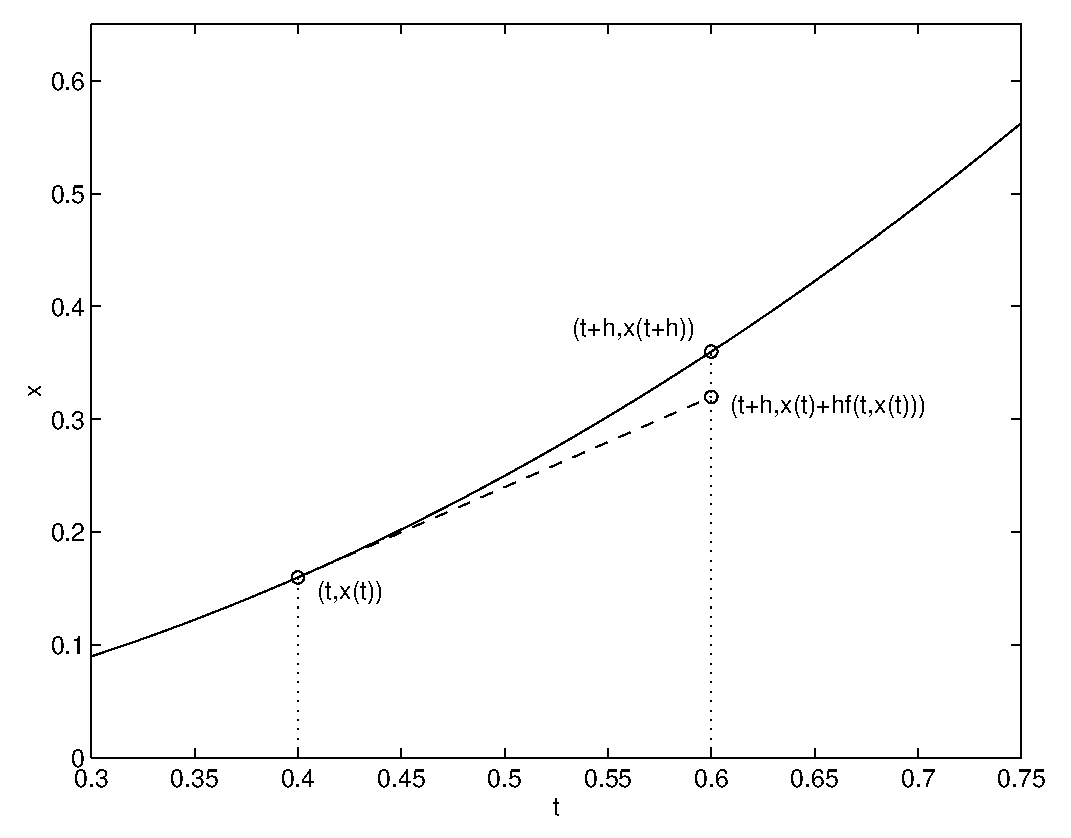
\psfig{file=../figures/eul1.eps,width=4.6in}}
   \caption{Illustration of one step in Euler's method
   for $h=0.2$.}
   \label{fig:eul1ill}
\end{figure*}

Concretely, Euler's method produces a sequence of approximations
to a solution of an initial value problem.  To understand this point, 
begin the numerical integration at the exact initial value $(t_0,x_0)$.  
Choose a {\em step size\/} \index{step size}
$h>0$.  Use \eqref{eq:eul1} to obtain after 
one {\em integration step\/} \index{integration step}
the approximation $x(t_1)\approx x_1$ where
\[
t_1 = t_0+h \AND x_1 = x_0 + h f(t_0, x_0).
\]
Continuing this process, construct a sequence
\begin{equation}  \label{eq:eulmethod}
t_{k+1} = t_k+h \AND x_{k+1} = x_k + h f(t_k, x_k)
\end{equation}
for $k=0,1,\ldots,K-1$ where $K$ is the total number of 
steps that are performed in the numerical approximation.

\subsubsection*{An Example of Euler's Method}
We illustrate how Euler's method works for the example
\arraystart
\begin{equation}  \label{eq:eulexivp}
\begin{array}{rcl}
\dps\frac{dx}{dt} & = & x+t\\
  x(1) & = & 2,
\end{array}
\end{equation}
\arrayfinish
by using \Matlab to compute an approximation to $x(3)$.  Suppose that we
set the step size to $h = 0.2$.  Then the number of steps needed to reach 
$t=3$ is $K=10$.  The code for computing the sequence in 
\eqref{eq:eulmethod} is:

\begin{verbatim}
h    = 0.2;
t(1) = 1;
x(1) = 2;
K    = 10;
for k = 1:K
   t(k+1) = t(k)+h;
   x(k+1) = x(k)+h*(x(k)+t(k));
end
plot(t,x,'o')
hold on
plot(t,x,'--')
xlabel('(a)')
\end{verbatim}\index{\computer!for\ldots end}\index{\computer!plot}
\index{\computer!hold}
The result is shown in Figure~\ref{fig:eulex1}(a).  Note that the
{\sf 'o'} in the \Matlab command {\tt plot(t,x,'o')} puts o's at the 11 
numerically computed points and the {\sf '-\,-'} in the command
{\tt plot(t,x,'--')} interpolates dashed lines between successive o's. 
Moreover, the statements within the {\tt for} loop --- that is the
lines from {\tt for k = 1:K} up to the {\tt end} --- 
reproduce the iteration procedure given in \eqref{eq:eulmethod}.
(In \Matlab the index of a vector is not allowed to be zero. Therefore, 
the {\tt for} loop is programmed to run from $k=1,\ldots,K$ rather than 
from $k=0,\ldots,K-1$.)

\subsubsection*{Comparison of Numerical Solutions with Exact Solutions}
\index{solution!numerical}\index{solution!exact}

We now compare the numerical approximation with the exact solution 
of \eqref{eq:eulexivp}, that is given by
\[
x(t) = 4e^{t-1}-t-1.
\]
This comparison is made in Figure~\ref{fig:eulex1}(b).  The second
curve in the figure is obtained using the additional commands
\begin{verbatim}
s = 1 : 0.01 : 3;
y = 4*exp(s-1)-s-1;  
plot(s,y)        
xlabel('(b)')
\end{verbatim}
Note that in that figure the scale on the vertical axis is
different from the one in Figure~\ref{fig:eulex1}(a).
\begin{figure*}[htb]
   \centerline{%
   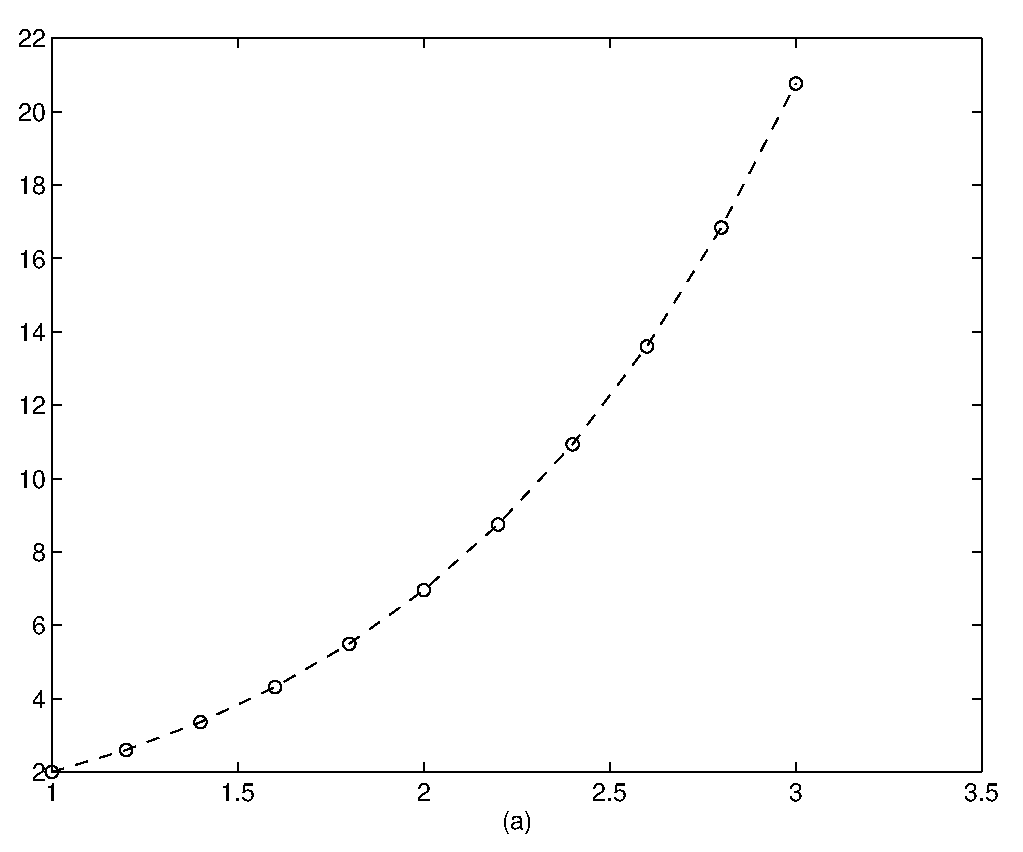
\psfig{file=../figures/eulex1.eps,width=3in}
   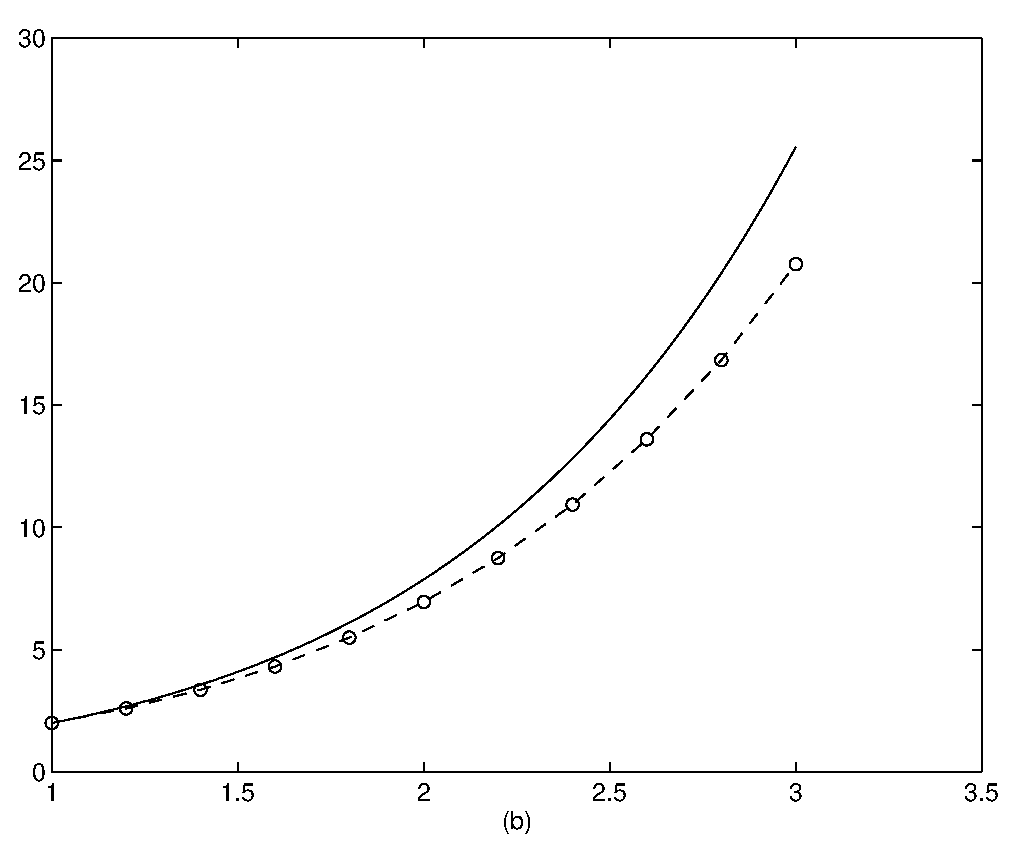
\psfig{file=../figures/eulex2.eps,width=3in}}
   \caption{Approximation of the solution of 
   \protect\eqref{eq:eulexivp} by Euler's method.  
   (a) Circles mark the computed points; dashed lines 
    are linear interpolations between the o's.  (b)  A comparison is 
    made to the exact solution pictured as a solid line.}
   \label{fig:eulex1}
\end{figure*}


In this example we see that after just $10$ steps the numerical solution 
of the initial value problem\index{initial value problem!numerical solution} 
by Euler's method has led to a significant 
error (see Figure~\ref{fig:eulex1} (b)).  There are two ways to proceed.
Either we can use a smaller step size\index{step size} in 
Euler's method in an attempt to 
improve accuracy or we can develop numerical methods that give more 
precise results for the same step size. For an illustration of the
first approach we show in Figure~\ref{fig:eulimpr}
an approximation with Euler's method using a step size
$h=0.05$.  It can be seen that the error is now indeed much smaller
but that also quite a few iterations of Euler's method are needed 
to produce this result.  Therefore the latter approach has 
generally proved preferable and one idea for improving accuracy is 
to replace $f(t_k,x_k)$ in the right hand side of 
\eqref{eq:eulmethod} by another expression in ways that we now explain.
\begin{figure}[htb]
   \centerline{%
   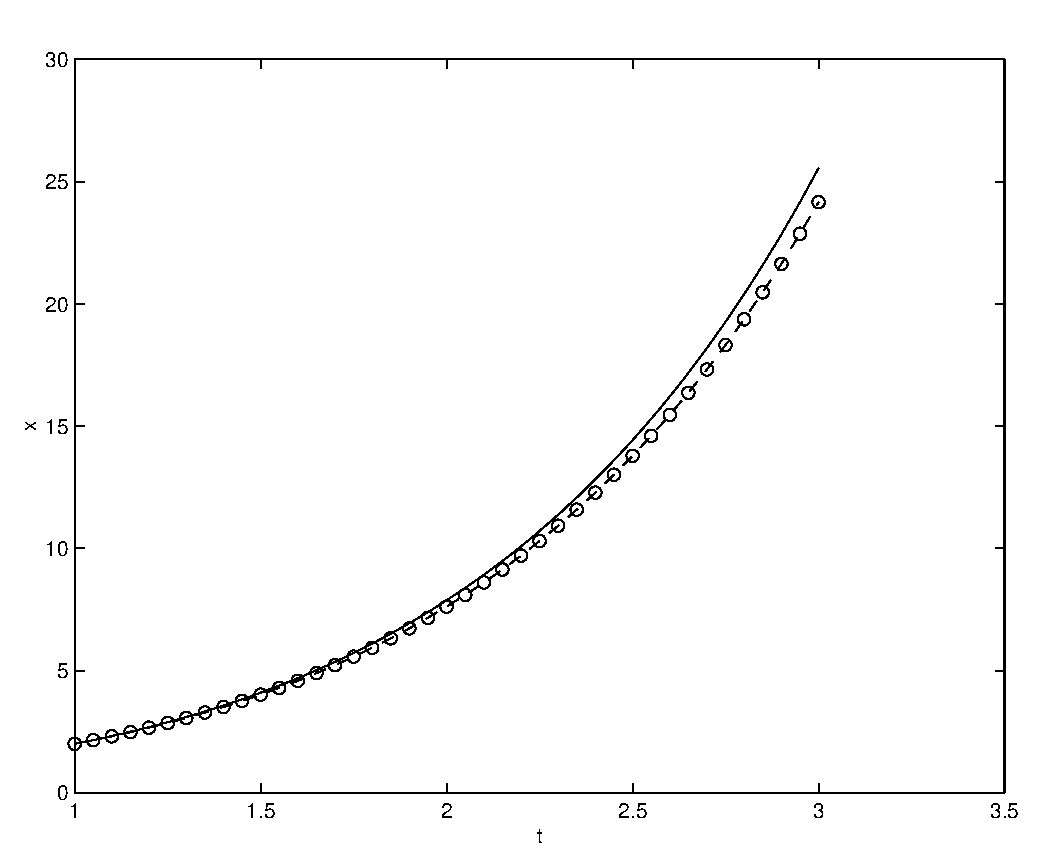
\psfig{file=../figures/eulimpr.eps,width=3.4in}}
   \caption{Approximation of the solution of
   \protect\eqref{eq:eulexivp} by Euler's method with step size
   $h=0.05$.  (Marks and lines as in Figure~\protect\ref{fig:eulex1}.)}
   \label{fig:eulimpr}
\end{figure}


\subsection*{Implicit Methods}  

In Euler's method, the approximation $x_{k+1}$ is computed using the 
tangent line to the graph of the solution at the point $(t_k,x_k)$.  
Another idea is to approximate the graph of $x(t)$ by the line passing 
through the point $(t_k,x_k)$ whose slope is $f(t_{k+1},x_{k+1})$.  
This idea leads to the numerical approximation
\[
t_{k+1} = t_k+h \AND x_{k+1} = x_k + h f(t_{k+1}, x_{k+1})
\]
which is known as the {\em implicit Euler method}.  
\index{implicit Euler method} \index{Euler's method!implicit}
One difficulty with 
this method is that we do not yet know what the value of $x_{k+1}$ is.
However, it is {\em implicitly\/} defined in the sense that
we can think of the iteration step 
\begin{equation}
\label{eq:impleulit}
x_{k+1} = x_k + h f(t_{k+1}, x_{k+1})
\end{equation}
as an equation in the unknown $x_{k+1}$ and use this nonlinear equation 
to solve for $x_{k+1}$.  We remark that there are
ODEs (e.g.\ so-called {\em stiff\/} equations) for which implicit 
schemes typically produce more reliable results.  On the other hand, 
implicit methods require considerable additional numerical effort at 
each time step in order to solve the equations for $x_{k+1}$. 

An implicit numerical method that is more accurate than implicit Euler 
is obtained by just averaging the Euler and implicit Euler 
approximations, to obtain
\begin{equation}
\label{eq:imtrap}
t_{k+1} = t_k+h \AND x_{k+1} = x_k + \frac{h}{2}
\Big( f(t_k, x_k)+f(t_{k+1}, x_{k+1})\Big).
\end{equation}
This method is called the {\em implicit trapezoidal rule}.  
\index{implicit trapezoidal rule}

\subsection*{The Modified Euler Method} \index{modified Euler method}
\index{Euler's method!modified}

As we discussed, the problem with implicit methods is that they require
the solution of a nonlinear equation at each time step.  In principle
this can also be done numerically, but such solutions 
require much numerical effort.  This problem can partly be overcome by 
using a clever idea discovered by {\sc Runge} (1895).  We illustrate 
this idea on the implicit trapezoidal rule.  Rather than determining 
$x_{k+1}$ directly from \eqref{eq:imtrap}, first estimate 
$x_{k+1}$ by $y_{k+1}$ using Euler's 
(tangent line) method.  Then use the estimate $y_{k+1}$ in the implicit 
trapezoidal rule\index{implicit trapezoidal rule}.
In formulas we obtain:
\[
t_{k+1} = t_k+h \AND
\left\{\begin{array}{rcl}
y_{k+1} & = & x_k + h f(t_k, x_k)\\
x_{k+1} & = & x_k + \frac{h}{2}
\Big( f(t_k, x_k)+f(t_{k+1}, y_{k+1})\Big),
\end{array}\right.
\]
or, in one line,
\begin{equation}
\label{eq:meulmethod}
t_{k+1} = t_k+h \AND
x_{k+1} = x_k + \frac{h}{2}
\Big( f(t_k, x_k)+f(t_{k+1}, x_k + h f(t_k, x_k))\Big).
\end{equation}
The resulting numerical method is called the {\em modified Euler method}.
\index{modified Euler method} \index{Euler's method!modified}

Let us use \Matlab to solve the initial value problem
\index{initial value problem!numerical solution}
\eqref{eq:eulexivp} by the modified Euler method.  
Using the same data as in the previous example we type
\begin{verbatim}
h    = 0.2;
t(1) = 1;
x(1) = 2;
K    = 10;
for k = 1:K
   t(k+1) = t(k)+h;
   y(k)   = x(k)+h*(x(k)+t(k));
   x(k+1) = x(k)+(h/2)*(x(k)+t(k)+y(k)+t(k+1));
end
plot(t,x,'o')
hold on
plot(t,x,'--')
s = 1 : 0.01 : 3;
y = 4*exp(s-1)-s-1;
plot(s,y)
xlabel('(a)')
\end{verbatim}
to obtain the illustration in Figure~\ref{fig:mEul}(a).
We see that the approximation can hardly be distinguished from
the exact solution.  Even if we double the step size\index{step size} 
to $h=0.4$ and reduce the number of steps to $K=5$, the 
approximation is still acceptable.  See Figure~\ref{fig:mEul}(b).

\begin{figure*}[htb]
   \centerline{%
   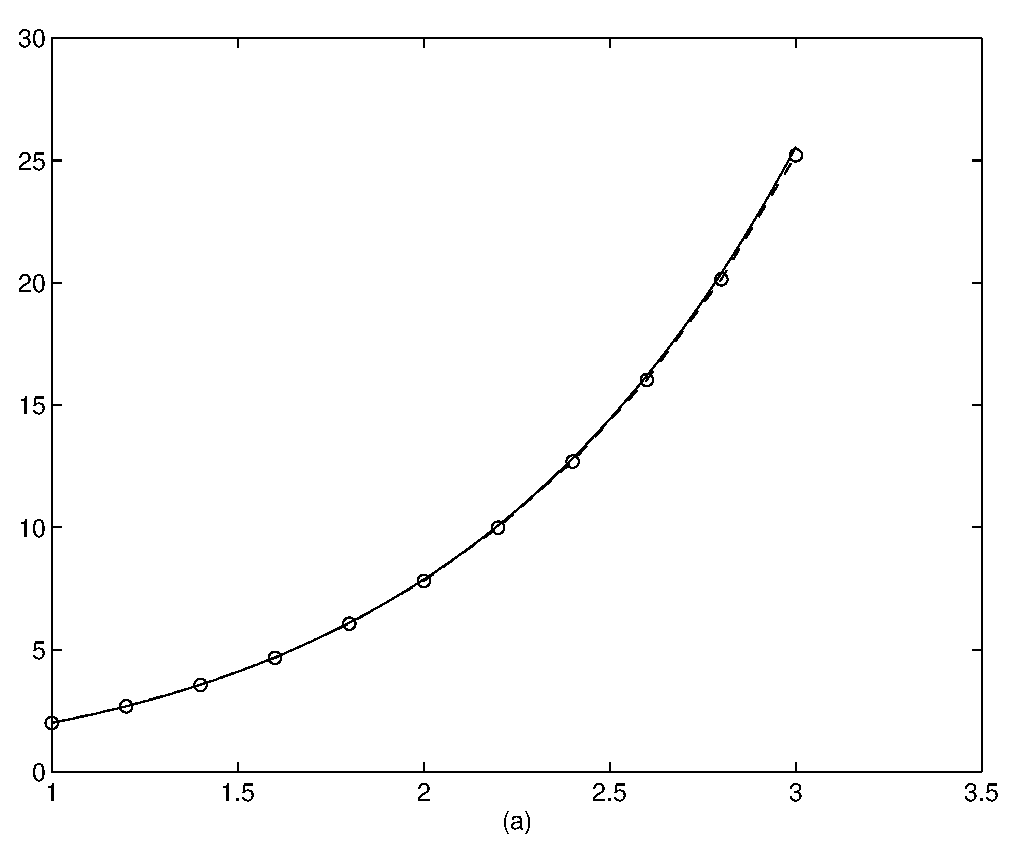
\psfig{file=../figures/meul1.eps,width=3in}
   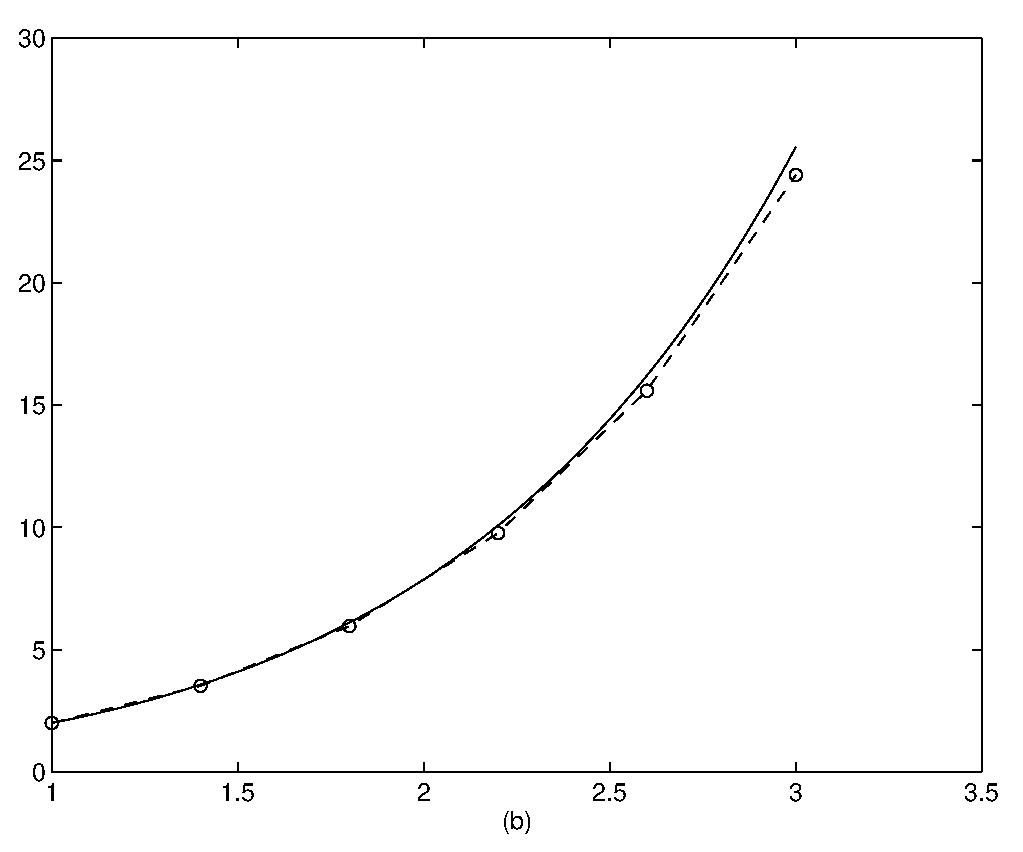
\psfig{file=../figures/meul2.eps,width=3in}}
   \caption{Approximations of the solution of
   \protect\eqref{eq:eulexivp} by the modified Euler method
   with step sizes: (a) $h=0.2$; (b) $h=0.4$.
   The exact solution is shown with a solid line.}
   \label{fig:mEul}
\end{figure*}

\subsection*{Fourth Order Runga-Kutta Method}
\index{fourth order Runge-Kutta method}
\index{Runge-Kutta method!fourth order}

The idea in the construction of the modified Euler method is to obtain a 
better approximation of the solution by using more information on the 
underlying differential equation.  This is realized in the scheme by 
taking the arithmetic average of two evaluations of the right hand side 
$f$ at different points rather than at just one point as in the 
standard Euler methods.

In the frequently used {\em fourth order Runge-Kutta method\/} four 
different evaluations of $f$ are taken into account in the computation of 
the next iterate.  The method is given as follows: set
\begin{eqnarray*}
f_1 &=& f(t_k,x_k)\\
f_2 &=& f\left(t_k+\frac{h}{2},x_k+\frac{h}{2}f_1\right)\\
f_3 &=& f\left(t_k+\frac{h}{2},x_k+\frac{h}{2}f_2\right)\\
f_4 &=& f(t_k+h,x_k+hf_3),
\end{eqnarray*}
and define the new approximation by
\[
x_{k+1} = x_k+\frac{h}{6}(f_1+2f_2+2f_3+f_4).
\]
By this method we can approximate solutions of differential equations
in a very precise way.  We illustrate this by an application to 
the initial value problem \eqref{eq:eulexivp}.  In Figure~\ref{fig:rk1} we
show the approximation obtained with the step size $h=0.6$ for $K=20$
steps.  The result is particularly convincing --- observe that
in contrast to Figures~\ref{fig:eulex1}--\ref{fig:mEul} the solution is
approximated on a significantly larger interval.
\begin{figure}[htb]
   \centerline{%
   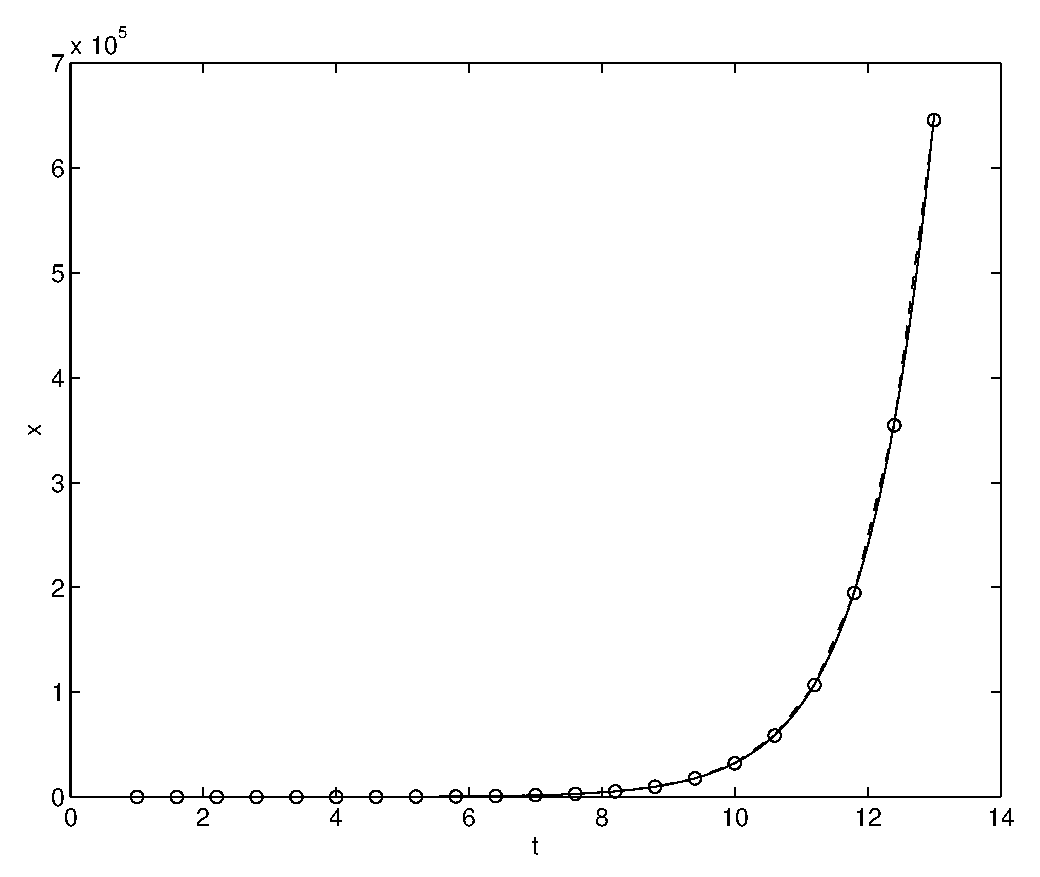
\psfig{file=../figures/runkut1.eps,width=3.6in}}
   \caption{Approximation of the solution of
   \protect\eqref{eq:eulexivp} obtained by the fourth order Runge-Kutta
   method.  The exact solution is superimposed (solid line).}
   \label{fig:rk1}
\end{figure}

\subsection*{Systems of Differential Equations}

All the methods we have introduced in this section can
also be used to find numerically solutions of systems 
of differential equations.  We illustrate this fact for
systems of two equations using Euler's method.

In the scalar case the underlying idea for 
Euler's method\index{Euler's method} was 
to approximate the solution of the differential equation over 
a short interval by a line that is tangent to the solution curve
(see Figure~\ref{fig:eul1ill}).  We now use the same approach 
by applying this idea to each component of the solution.

Suppose that $(x(t),y(t))$ is a solution of the initial value problem
\arraystart
\begin{equation}
\label{eq:numanalsys}
\begin{array}{rcl}
\dps \frac{dx}{dt} & = & f(t,x,y)\\
\dps \frac{dy}{dt} & = & g(t,x,y),
\end{array}
\end{equation}
\arrayfinish
where $(x(t_0),y(t_0))= (x_0,y_0)$.  As in \eqref{eq:eul1}
we obtain for the components $x(t)$ and $y(t)$
by using the differential equation 
\begin{eqnarray*}
x(t+h) & \approx & x(t) + h \frac{dx}{dt}(t) = x(t) + h f(t,x(t),y(t))\\
y(t+h) & \approx & y(t) + h \frac{dy}{dt}(t) = y(t) + h g(t,x(t),y(t)).
\end{eqnarray*}
Again $h>0$ is called the step size\index{step size}.
We can now proceed as in the case of a scalar differential equation 
and obtain in analogy to \eqref{eq:eulmethod} 
\begin{eqnarray*}
t_{k+1} = t_k+h \AND 
\left\{\begin{array}{rcl}
x_{k+1} &=& x_k + h f(t_k,x_k,y_k)\\
y_{k+1} &=& y_k + h g(t_k,x_k,y_k)
\end{array}\right.
\quad (k=0,1,\ldots,K-1).
\end{eqnarray*}
Using vector notation Euler's method applied to the initial value problem
\eqref{eq:numanalsys} can be written as
\arraystart
\begin{equation}
\begin{array}{rcl}
\vectwo{x_{k+1}}{y_{k+1}} & = & 
\vectwo{x_k}{y_k} + h \vectwo{f(t_k,x_k,y_k)}{g(t_k,x_k,y_k)}\\
t_{k+1} & = & t_k + h,
\end{array}
\end{equation}
\arrayfinish
for $k=0,1,\ldots,K$.

Similarly, the implicit Euler 
method\index{Euler's method!implicit}\index{implicit Euler method} 
takes the form
\begin{eqnarray*}
\vectwo{x_{k+1}}{y_{k+1}} & = &  \vectwo{x_k}{y_k} + 
h \vectwo{f(t_{k+1},x_{k+1},y_{k+1})}{g(t_{k+1},x_{k+1},y_{k+1})}\\
t_{k+1} &=& t_k + h.
\end{eqnarray*}
Let us use \Matlab to compute an approximation of the initial
value problem
\arraystart
\begin{equation}
\label{eq:numanalex1}
\begin{array}{rcl}
\dps \frac{dx}{dt} & = & y-3t\\
\dps \frac{dy}{dt} & = & y+x^2,
\end{array}
\end{equation}
\arrayfinish
where $(x(1),y(1))= (0,2)$.  We specify the 
step size $h=0.05$ and find an approximation on the interval 
$[1,3]$ by typing
\begin{verbatim}
h    = 0.05;
t(1) = 1;
x(1) = 0;
y(1) = 2;
K    = 40;
for k = 1:K
   t(k+1) = t(k)+h;
   x(k+1) = x(k)+h*(y(k)-3*t(k));
   y(k+1) = y(k)+h*(y(k)+x(k)^2);
end
plot(x,y,'o')
hold on
plot(x,y,'--')
xlabel('x')
ylabel('y')
\end{verbatim}\index{\computer!for\ldots end}\index{\computer!plot}
\index{\computer!hold}
The result is shown in Figure~\ref{fig:sysEul1}.
\begin{figure}[htb]
   \centerline{%
   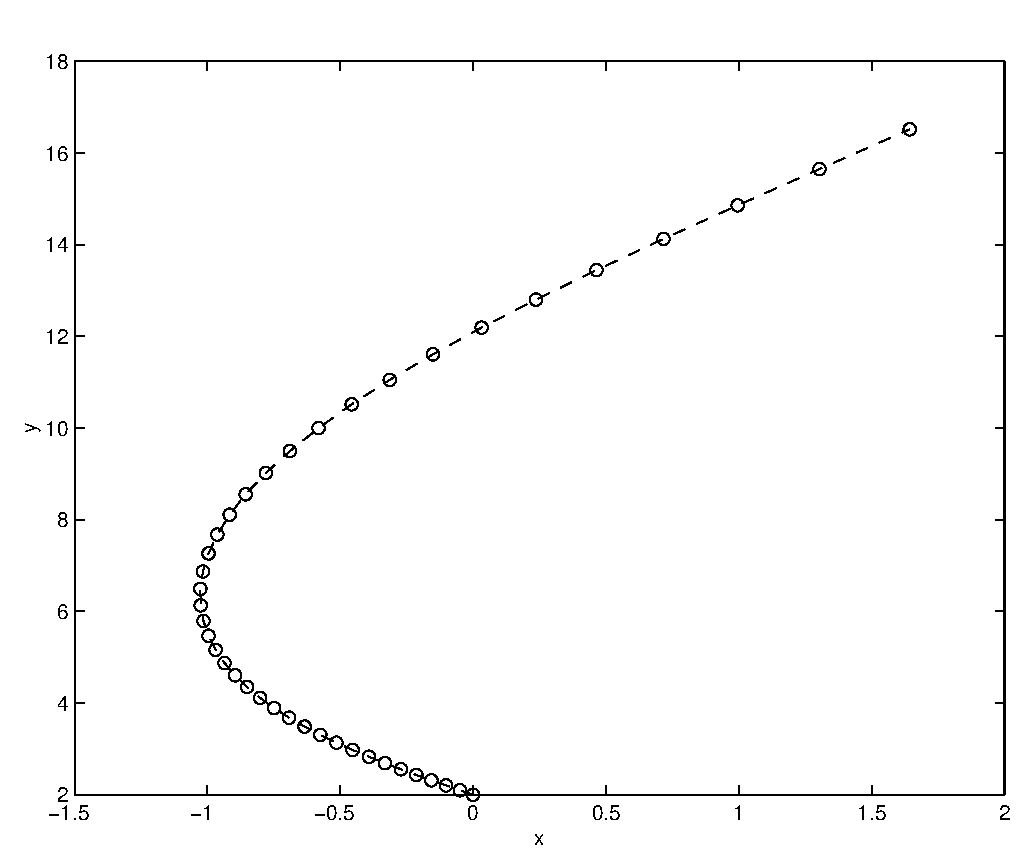
\psfig{file=../figures/eulsys1.eps,width=3.6in}}
   \caption{Approximation of the solution of
   \protect\eqref{eq:numanalex1} by Euler's method
   with step size $h=0.05$.  The single points of
   the approximation are marked by circles.}
   \label{fig:sysEul1}
\end{figure}
Observe that the solution $(x(t),y(t))$ is graphed in
the $xy$-plane.
In particular, the variable $t$ does not appear in the figure 
and this is the reason why the single steps in the approximation
do not seem to be equally spaced.  However, in
Figure~\ref{fig:sysEul2} we show graphs of the approximations
of the time series $x$ vs.\ $t$ and $y$ vs.\ $t$. Here 
it can be seen that the step size is indeed constant.
\begin{figure*}[htb]
   \centerline{%
   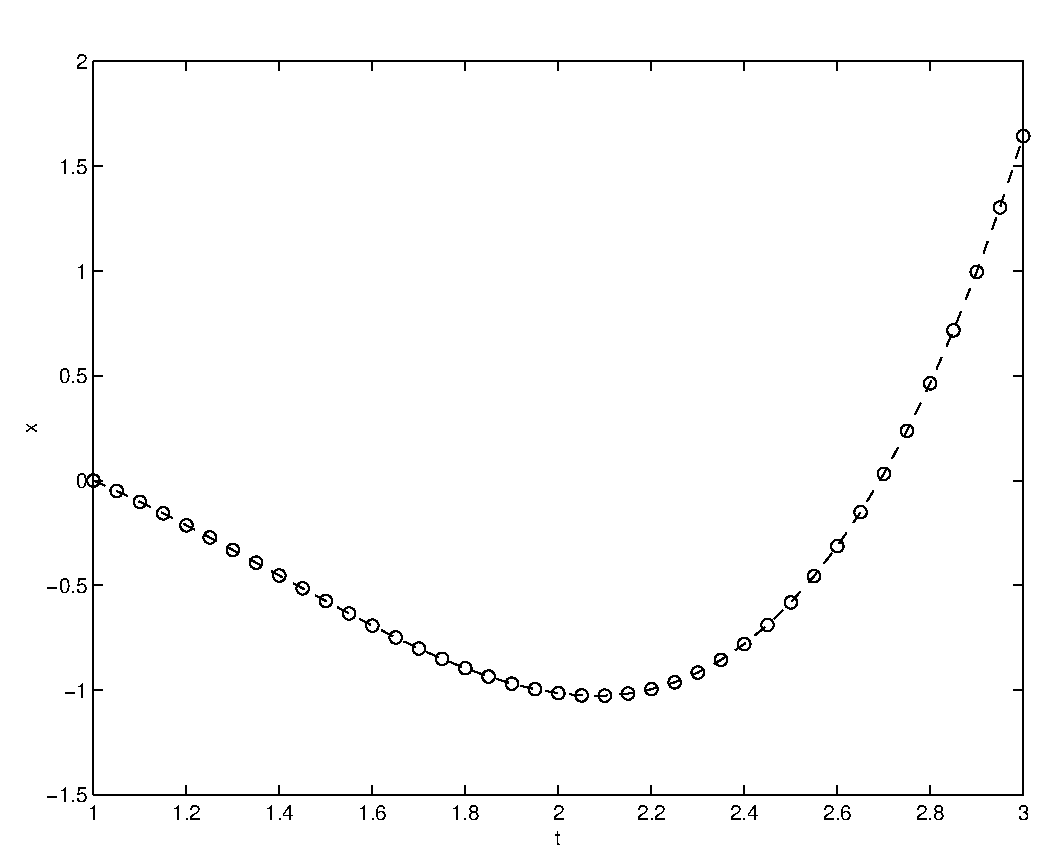
\psfig{file=../figures/eulsys2.eps,width=3in}
   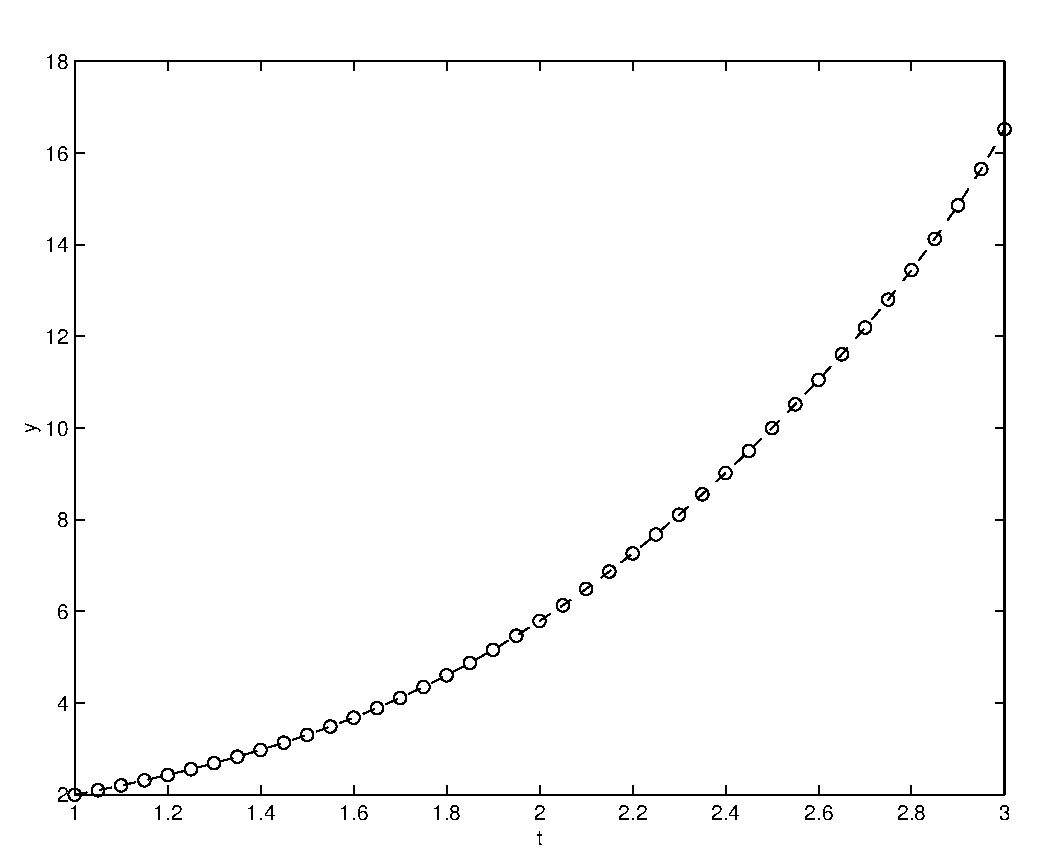
\psfig{file=../figures/eulsys3.eps,width=3in}}
   \caption{Approximation of the $x$- and $y$-components
   of the solution of \protect\eqref{eq:numanalex1} by Euler's method
   with step size $h=0.05$.}
   \label{fig:sysEul2}
\end{figure*}


There are several ways to improve the accuracy of 
numerical schemes approximating solutions of initial value problems. 
One very successful method is to adapt the step size $h$ in each
step of the numerical approximation.  We illustrate this
strategy in Appendix~\ref{sec:appslc}.


\subsection*{General Runga-Kutta Methods}
\index{Runge-Kutta method!general}

The modified Euler method as well as the fourth order Runge-Kutta
method are specific examples of a general class of 
numerical schemes for the solution of initial value 
problems\index{initial value problem!numerical solution}.
These schemes are called {\em Runge-Kutta methods}.  A general explicit 
Runge-Kutta method is fully described by numbers
\[
b_1,\ldots,b_s\AND c_1,\ldots,c_s,
\]
and 
\[
a_{pq}, \quad p=2,\ldots,s,\quad q=1,\ldots,p-1.
\]
With these numbers the $k^{th}$ step in the numerical solution of an 
initial value problem using a Runge-Kutta method can be described
as follows. Given $(t_k,x_k)$ first evaluate $f$ for $s$ times:
\begin{eqnarray*}
f_1 & = & f\left( t_k+c_1 h, x_k \right)\\
f_2 & = & f\left( t_k+c_2 h, x_k +ha_{21} f_1\right)\\
f_3 & = & f\left( t_k+c_3 h, x_k +h(a_{31} f_1 + a_{32} f_2)\right)\\
& \vdots &\\
f_s & = & f\left( t_k+c_s h, x_k +h\sum_{j=1}^{s-1}a_{ij} f_j\right).
\end{eqnarray*}
Second, obtain the next approximation by a weighted average
of $f_1,\ldots,f_s$:
\[
t_{k+1} = t_k+h \AND x_{k+1} = x_k + h\sum_{i=1}^s b_i f_i.
\]
We now show that --- except for the implicit schemes ---
all the methods that we have discussed are Runge-Kutta methods.

\begin{itemize}
\item[(a)] {\em Euler's method:} 
\index{Euler's method}
set
\[
s=1,\quad b_1=1,\quad c_1=0 
\]
and there are no $a_{pq}$'s.
\item[(b)] {\em The modified Euler method:} 
\index{modified Euler method} set
\[
s=2,\quad b_1=b_2=1/2,\quad c_1=0,\quad c_2=1,\quad a_{21}=1.
\]
Indeed, using these data
\begin{eqnarray*}
f_1 &=& f(t_k,x_k)\\
f_2 &=& f(t_{k+1},x_k+hf_1)=f(t_{k+1},x_k+hf(t_k,x_k)),
\end{eqnarray*}
and
\begin{eqnarray*}
x_{k+1} &=& x_k + h \left(\frac{1}{2}f_1 + \frac{1}{2}f_2\right)\\
&=& x_k + \frac{h}{2}
\Big( f(t_k, x_k)+f(t_{k+1}, x_k + h f(t_k, x_k))\Big).
\end{eqnarray*}
Hence we have obtained \eqref{eq:meulmethod}.
\item[(c)] {\em Fourth order Runge-Kutta method:} 
\index{fourth order Runge-Kutta method}
\index{Runge-Kutta method!fourth order}
set 
\[
s=4,\quad b_1=b_4=1/6,\quad b_2=b_3=2/6,\quad 
c_1=0,\quad c_2=c_3=1/2,\quad c_4=1,
\]
and 
\[
a_{21}=1/2,\quad a_{31}=0,\quad a_{32}=1/2,\quad
a_{41}=0,\quad a_{42}=0,\quad a_{43}=1.
\]
\end{itemize}


\EXER

\includeexercises

\end{document}
